\documentclass{article}
\usepackage{ listings} 
\usepackage{amsmath}
\usepackage{float} 
\usepackage{graphicx}
\usepackage{subcaption}
\usepackage{geometry}
\usepackage{amsthm}
\usepackage{amssymb}

\begin{document}
\title{Solution to Homework 4}
\author{Shoeb Mohammed and Zhuo Chen}
\maketitle

\newcommand{\QEDA}{\hfill\ensuremath{\blacksquare}}
\newcommand{\QEDB}{\hfill\ensuremath{\square}}

\section{Kernelizing the perceptron}
\begin{equation*}
	\mathcal{D} = \{x^{(i)} | 1 \leq i \leq m\, y^{(i)} \in \{-1,1\}\} 
\end{equation*}

\begin{equation}
	\label{eq:1.1}
    \theta^{(i)} \leftarrow \theta^{(i-1)} - [h_{\theta^{(i-1)}}(x^{(i)}) - y^{(i)}]x^{(i)}
\end{equation}

\subsection{}
From equation~\ref{eq:1.1}, it is clear that $\theta$ is a linear combination of vectors $x^{(i)}$.
Thus, $\theta$ can be implicitly represented by the weights $\alpha_i$ in
\begin{equation}
	\label{eq:1.2}
    \theta = \sum_{i=1}^{m} \alpha_i \phi(x^{(i)})
\end{equation}
The $\alpha_i$ are dual variables and initialized to zero.

\subsection{}
From equation~\ref{eq:1.2} it follows that
\begin{equation}
  \label{eq:1.3}
  \begin{split}
  h_{\theta^{(i)}}(\phi(x^{(i+1)})) &= sign\left(\theta^{(i)^T}\phi(x^{(i+1)})\right) \\
                  &= sign\left(\sum_{j=1}^{m} \alpha_j \phi(x^{(j)})^T \phi(x^{(i+1)})\right) \\
				  &= sign\left(\sum_{j=1}^{m} \alpha_j K( x^{(j)}, x^{(i+1)} )\right)
  \end{split}
\end{equation}
In equation~\ref{eq:1.3}, during training, $\alpha_j = 0$ for $j > i$.


\subsection{}
For a new training example, we use the update rule
\begin{equation}
  \label{eq:1.4}
  \begin{split}
   \alpha_{i+1} &\leftarrow h_{\theta^{(i)}}(\phi(x^{(i+1)})) - y^{(i)} \\
   			&\leftarrow sign\left(\sum_{j=1}^{m} \alpha_j K( x^{(j)}, x^{(i+1)} )\right) - y^{(i)}
  \end{split}
\end{equation}
In equation~\ref{eq:1.4}, during training, $\alpha_j = 0$ for $j > i$.


\section{Fitting an SVM classifier by hand}
\begin{equation*}
	\mathcal{D} = \{ (0,-1) , (\sqrt{2},+1) \} 
\end{equation*}
\begin{equation*}
	\phi(x) = (0,\sqrt{2}x,x^2) 
\end{equation*}
We fit a maximum margin classifier for $\mathcal{D}$ and features $\phi(x)$.

\subsection{}
The vector $v$ along the line joining the two points is parallel to optimal vector $\theta$.
\begin{equation*}
	v = (0,2,2)
\end{equation*}

\subsection{}
The value of the margin is $2\sqrt{2}$.

\subsection{}
\begin{equation*}
	\theta = (0,1,1)
\end{equation*}

\subsection{}
\begin{equation*}
	\theta_0 = 2
\end{equation*}

\subsection{}
The equation for decision boundary is
\begin{equation*}
	\theta^T \phi(x) = 2
\end{equation*}

\section{Support vector machines for binary classification}

\subsection{Support vector machines}
\subsubsection{The hinge loss function and gradient}
\subsubsection{Example dataset 1: impact of varying C}
\begin{itemize}
	\item Checked loss function and gradient with the values in the homework.
	\item Verified decision boundary with C=100. It matches the boundary in homework figure 3.
\end{itemize}

\subsubsection{Gaussian kernel}
\begin{itemize}
	\item Implemented the Gaussian kernel.
	\item Verified it works correct.
	\item The decision boundary using Gaussian kernel is plotted in figure~\ref{fig:3.1_gb}
\end{itemize}

\begin{figure}[H]
	\centering
	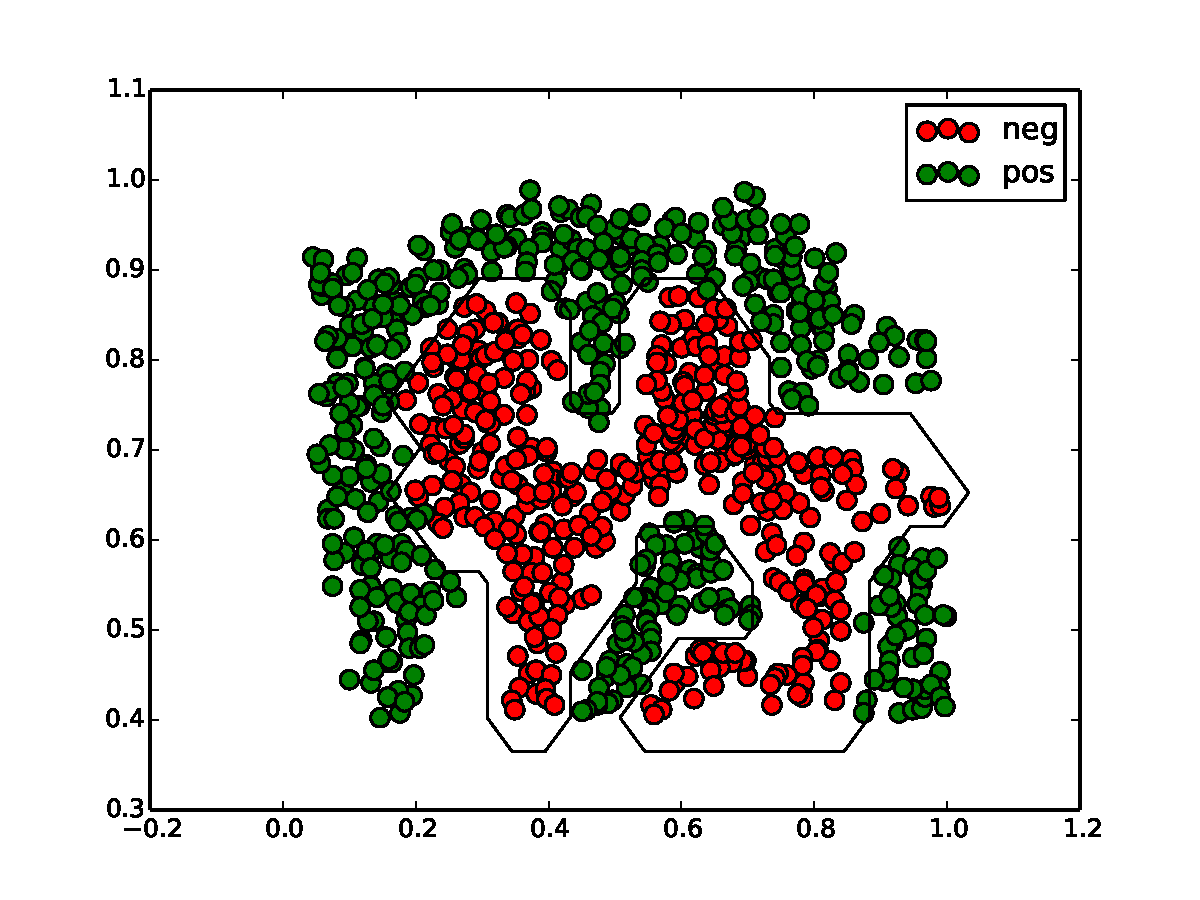
\includegraphics[width=1\linewidth]{./fig4}
	\caption{Learning non-linear boundary using a Gaussian kernel}\label{fig:3.1_gb}
\end{figure}

\subsection{Example dataset 3: selecting hyper parameters for SVMs}
Searching over $C,\sigma \in \{0.01,0.03,0.1,0.3,1,3,10,30\}$ we get following best hyper parameters.
The decision boundary is plotted in figure~\ref{fig:3.2}
\begin{lstlisting}
	*****Problem 3.2******
	Best C = 1.000000e-01 Best sigma = 1.000000e-01
	with validation accuracy = 9.600000e-01
\end{lstlisting}

\begin{figure}[H]
	\centering
	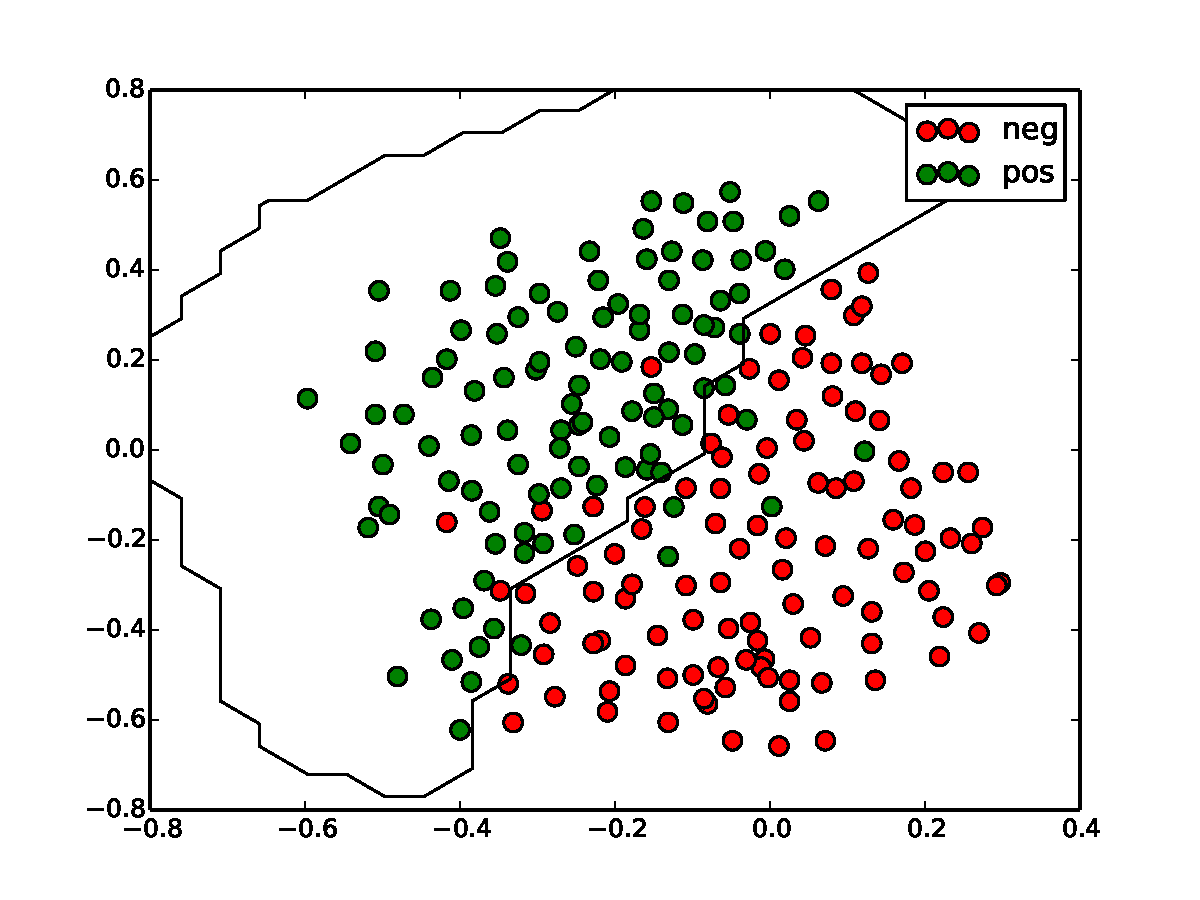
\includegraphics[width=1\linewidth]{./fig6}
	\caption{decision boundary with best $C=0.01$ and best $\sigma = 0.01$}\label{fig:3.2}
\end{figure}


\subsection{Spam Classification with SVMs}

\end{document}
